
%(BEGIN_QUESTION)
% Copyright 2010, Tony R. Kuphaldt, released under the Creative Commons Attribution License (v 1.0)
% This means you may do almost anything with this work of mine, so long as you give me proper credit

Sketch the proper tube and wire connections to calibrate this electronic DP transmitter to a range of 0 to 40 inches water column using a manometer as the pressure standard, and a multimeter to sense its 4-20 mA current output (registering a positive value for current).  Connect the three 6-volt batteries together to create an 18 volt power source:

$$\includegraphics[width=15.5cm]{i01378x01.eps}$$

\underbar{file i01378}
%(END_QUESTION)





%(BEGIN_ANSWER)

This is not the only correct solution.  The manometer connections may be reversed and still function perfectly.  The ammeter may be placed either before or after the transmitter in the series circuit:

$$\includegraphics[width=15.5cm]{i01378x02.eps}$$

-5 points if the multimeter registers the wrong polarity.  No points at all if the circuit will not function as sketched.

%(END_ANSWER)





%(BEGIN_NOTES)

{\bf This question is intended for exams only and not worksheets!}.

%(END_NOTES)

